\documentclass{standalone}
\usepackage{tikz}
\usetikzlibrary{patterns, positioning}
\usepackage[sfdefault]{ClearSans} %% option 'sfdefault' activates Clear Sans as the default text font
\usepackage[T1]{fontenc}

\begin{document}
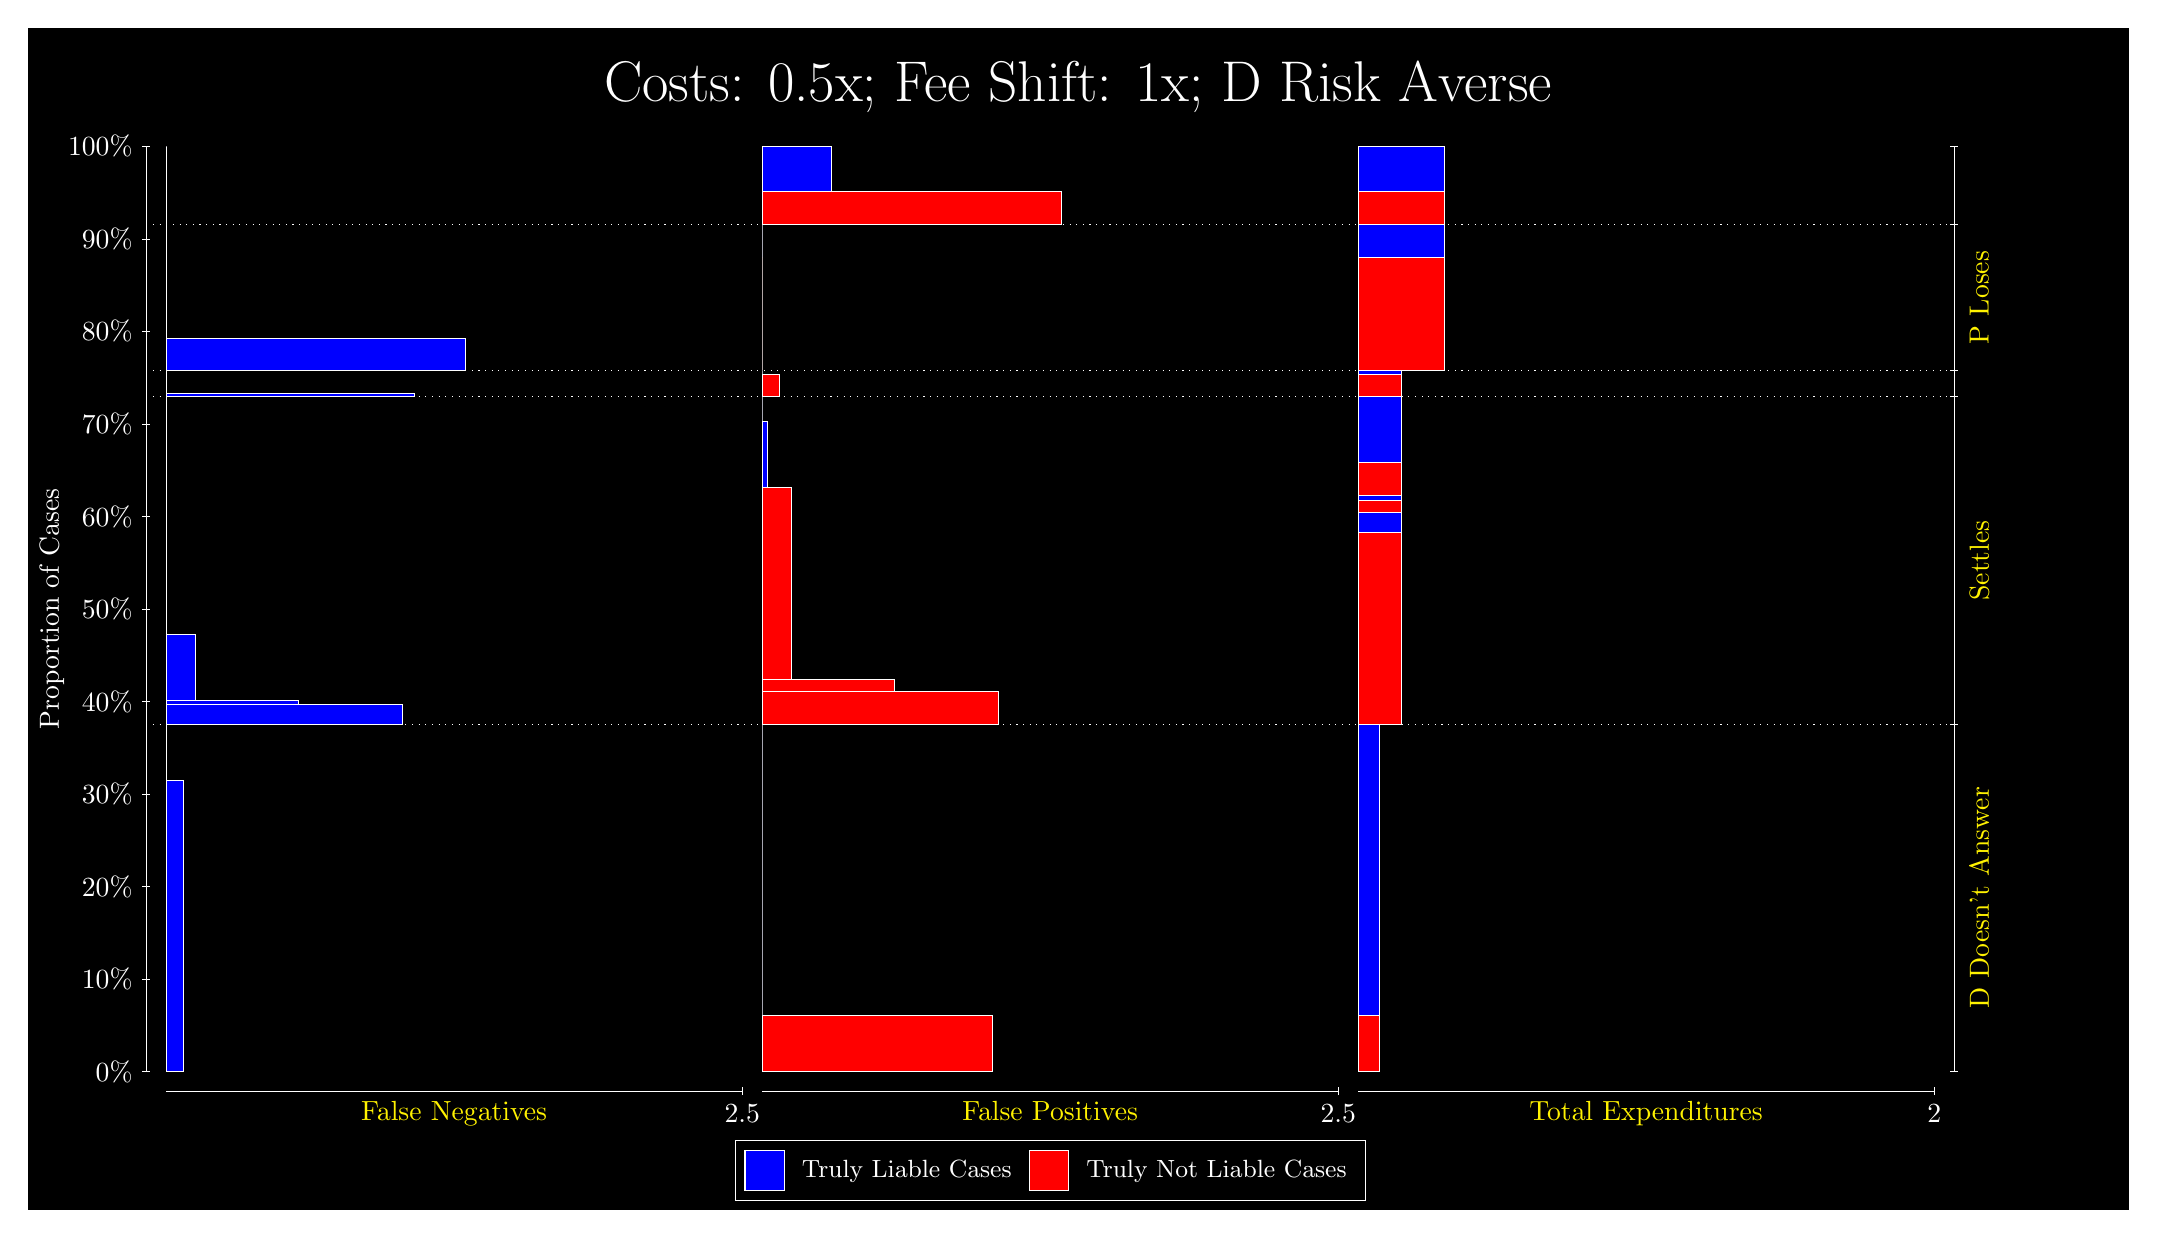
\begin{tikzpicture}
\draw[fill=black] (0,0) rectangle (26.667,15);
\draw[text=white] (0,13.5) rectangle (26.667,15) node[midway] {\huge Costs: 0.5x; Fee Shift: 1x; D Risk Averse};
\draw[white, very thin] (1.5,1.75) -- (1.5,13.5);
\node[rotate=90, text=white, anchor=center] at (0.3, 7.625) {Proportion of Cases};
\draw[white, very thin] (1.45,1.75) -- (1.55,1.75);
\node[text=white, anchor=east] at (1.45, 1.75) {0\%};
\draw[white, very thin] (1.45,2.925) -- (1.55,2.925);
\node[text=white, anchor=east] at (1.45, 2.925) {10\%};
\draw[white, very thin] (1.45,4.1) -- (1.55,4.1);
\node[text=white, anchor=east] at (1.45, 4.1) {20\%};
\draw[white, very thin] (1.45,5.275) -- (1.55,5.275);
\node[text=white, anchor=east] at (1.45, 5.275) {30\%};
\draw[white, very thin] (1.45,6.45) -- (1.55,6.45);
\node[text=white, anchor=east] at (1.45, 6.45) {40\%};
\draw[white, very thin] (1.45,7.625) -- (1.55,7.625);
\node[text=white, anchor=east] at (1.45, 7.625) {50\%};
\draw[white, very thin] (1.45,8.8) -- (1.55,8.8);
\node[text=white, anchor=east] at (1.45, 8.8) {60\%};
\draw[white, very thin] (1.45,9.975) -- (1.55,9.975);
\node[text=white, anchor=east] at (1.45, 9.975) {70\%};
\draw[white, very thin] (1.45,11.15) -- (1.55,11.15);
\node[text=white, anchor=east] at (1.45, 11.15) {80\%};
\draw[white, very thin] (1.45,12.325) -- (1.55,12.325);
\node[text=white, anchor=east] at (1.45, 12.325) {90\%};
\draw[white, very thin] (1.45,13.5) -- (1.55,13.5);
\node[text=white, anchor=east] at (1.45, 13.5) {100\%};

\draw[white, very thin] (24.457,1.75) -- (24.457,13.5);
\draw[white, very thin] (24.407,1.75) -- (24.507,1.75);
\node[anchor=west] at (24.407, 1.75) {};
\draw[white, very thin] (24.407,6.159) -- (24.507,6.159);
\node[anchor=west] at (24.407, 6.159) {};
\draw[white, very thin] (24.407,10.321) -- (24.507,10.321);
\node[anchor=west] at (24.407, 10.321) {};
\draw[white, very thin] (24.407,10.65) -- (24.507,10.65);
\node[anchor=west] at (24.407, 10.65) {};
\draw[white, very thin] (24.407,12.511) -- (24.507,12.511);
\node[anchor=west] at (24.407, 12.511) {};
\draw[white, very thin] (24.407,13.5) -- (24.507,13.5);
\node[anchor=west] at (24.407, 13.5) {};

\draw[white, very thin, fill=blue] (1.75,1.75) rectangle (1.9696,5.4494);
\draw[white, very thin, fill=red] (1.75,5.4494) rectangle (1.75,6.159);
\draw[white, very thin, fill=blue] (1.75,6.159) rectangle (4.7507,6.4139);
\draw[white, very thin, fill=blue] (1.75,6.4139) rectangle (3.4333,6.467);
\draw[white, very thin, fill=blue] (1.75,6.467) rectangle (2.1159,7.3037);
\draw[white, very thin, fill=red] (1.75,7.3037) rectangle (1.75,10.321);
\draw[white, very thin, fill=blue] (1.75,10.321) rectangle (4.8971,10.364);
\draw[white, very thin, fill=red] (1.75,10.364) rectangle (1.75,10.65);
\draw[white, very thin, fill=blue] (1.75,10.65) rectangle (5.5558,11.068);
\draw[white, very thin, fill=red] (1.75,11.068) rectangle (1.75,12.511);
\draw[white, very thin, fill=red] (1.75,12.511) rectangle (1.75,12.93);
\draw[white, very thin, fill=blue] (1.75,12.93) rectangle (1.75,13.5);
\draw[white, very thin, fill=red] (9.3189,1.75) rectangle (12.246,2.4595);
\draw[white, very thin, fill=blue] (9.3189,2.4595) rectangle (9.3189,6.159);
\draw[white, very thin, fill=red] (9.3189,6.159) rectangle (12.32,6.5799);
\draw[white, very thin, fill=red] (9.3189,6.5799) rectangle (11.002,6.7351);
\draw[white, very thin, fill=red] (9.3189,6.7351) rectangle (9.6848,9.176);
\draw[white, very thin, fill=blue] (9.3189,9.176) rectangle (9.3921,10.013);
\draw[white, very thin, fill=blue] (9.3189,10.013) rectangle (9.3189,10.321);
\draw[white, very thin, fill=red] (9.3189,10.321) rectangle (9.5384,10.607);
\draw[white, very thin, fill=blue] (9.3189,10.607) rectangle (9.3189,10.65);
\draw[white, very thin, fill=red] (9.3189,10.65) rectangle (9.3189,12.094);
\draw[white, very thin, fill=blue] (9.3189,12.094) rectangle (9.3189,12.511);
\draw[white, very thin, fill=red] (9.3189,12.511) rectangle (13.125,12.93);
\draw[white, very thin, fill=blue] (9.3189,12.93) rectangle (10.197,13.5);
\draw[white, very thin, fill=red] (16.888,1.75) rectangle (17.162,2.4595);
\draw[white, very thin, fill=blue] (16.888,2.4595) rectangle (17.162,6.159);
\draw[white, very thin, fill=red] (16.888,6.159) rectangle (17.437,8.5999);
\draw[white, very thin, fill=blue] (16.888,8.5999) rectangle (17.437,8.8548);
\draw[white, very thin, fill=red] (16.888,8.8548) rectangle (17.437,9.0101);
\draw[white, very thin, fill=blue] (16.888,9.0101) rectangle (17.437,9.0631);
\draw[white, very thin, fill=red] (16.888,9.0631) rectangle (17.437,9.484);
\draw[white, very thin, fill=blue] (16.888,9.484) rectangle (17.437,10.321);
\draw[white, very thin, fill=red] (16.888,10.321) rectangle (17.437,10.607);
\draw[white, very thin, fill=blue] (16.888,10.607) rectangle (17.437,10.65);
\draw[white, very thin, fill=red] (16.888,10.65) rectangle (17.986,12.094);
\draw[white, very thin, fill=blue] (16.888,12.094) rectangle (17.986,12.511);
\draw[white, very thin, fill=red] (16.888,12.511) rectangle (17.986,12.93);
\draw[white, very thin, fill=blue] (16.888,12.93) rectangle (17.986,13.5);
\draw[white, dotted] (1.5,6.159) -- (24.457,6.159);
\draw[white, dotted] (1.5,10.321) -- (24.457,10.321);
\draw[white, dotted] (1.5,10.65) -- (24.457,10.65);
\draw[white, dotted] (1.5,12.511) -- (24.457,12.511);
\draw[white, very thin] (1.75,1.5) -- (9.0689,1.5);
\node[text=yellow, anchor=north] at (5.4094, 1.5) {False Negatives};
\draw[white, very thin] (9.0689,1.45) -- (9.0689,1.55);
\node[text=white, anchor=north] at (9.0689, 1.45) {2.5};

\draw[white, very thin] (9.3189,1.5) -- (16.638,1.5);
\node[text=yellow, anchor=north] at (12.978, 1.5) {False Positives};
\draw[white, very thin] (16.638,1.45) -- (16.638,1.55);
\node[text=white, anchor=north] at (16.638, 1.45) {2.5};

\draw[white, very thin] (16.888,1.5) -- (24.207,1.5);
\node[text=yellow, anchor=north] at (20.547, 1.5) {Total Expenditures};
\draw[white, very thin] (24.207,1.45) -- (24.207,1.55);
\node[text=white, anchor=north] at (24.207, 1.45) {2};

\node[text=yellow, centered, rotate=90] at (24.777, 3.9545) {D Doesn't Answer};
\node[text=yellow, centered, rotate=90] at (24.777, 8.2398) {Settles};

\node[text=yellow, centered, rotate=90] at (24.777, 11.581) {P Loses};


\draw (12.978300999999998,1.5) node[draw=none] (baseCoordinate) {};
\begin{scope}[align=center]
        \matrix[scale=0.5, draw=white, below=0.5cm of baseCoordinate, nodes={draw}, column sep=0.1cm]{
            \node[rectangle, draw, minimum width=0.5cm, minimum height=0.5cm, fill=blue] {}; &
            \node[draw=none, font=\small, text=white] (B) {Truly Liable Cases}; &
            \node[rectangle, draw, minimum width=0.5cm, minimum height=0.5cm, fill=red] {}; &
            \node[draw=none, font=\small, text=white] (B) {Truly Not Liable Cases}; \\
            };
\end{scope}

\end{tikzpicture}
\end{document}